\documentclass[tikz]{standalone}
\usepackage{multicol}
\usepackage{pgfplots}
\usetikzlibrary{positioning}
\pgfplotsset{every axis legend/.append style={fill=none, draw=none}}
\pgfplotsset{compat=1.3}

\begin{document}
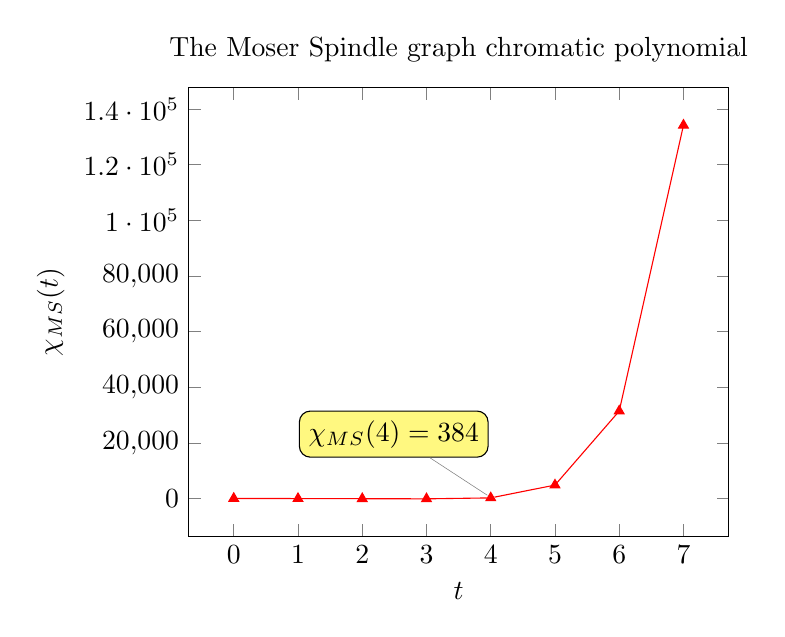
\begin{tikzpicture}
\tikzset{
  every pin/.style={fill=yellow!50!white, rectangle, draw, rounded corners},
  small dot/.style={fill=white, circle, scale=0.3}
}
\begin{axis}[
  title={The Moser Spindle graph chromatic polynomial},
  samples at={0,1,2,3,4,5,6,7},
  xlabel=$t$,
  ylabel=$\chi_{MS}(t)$,
  scaled ticks=false,
  try min ticks = 10,
  clip=false
]
\addplot[red, domain=1:7, mark=triangle*] {x^7 - 11*x^6 + 51*x^5 - 129*x^4 + 188*x^3- 148*x^2+ 48};

\node[small dot, pin=93:{$\chi_{MS}(4) = 384$}] at (axis cs:4,384) {};
\end{axis}
\end{tikzpicture}
\end{document}